\documentclass[class=scrbook, crop=false]{standalone}
\usepackage[subpreambles=true]{standalone}
\ifstandalone
    % WARNING: Proceed with caution!

% -----------------------------------------------------------------------------------
% For package standalone
% -----------------------------------------------------------------------------------
\usepackage{import}

% -----------------------------------------------------------------------------------
% Language and typeset
% -----------------------------------------------------------------------------------
\usepackage[ngerman, english]{babel}

\usepackage{subcaption}
% Umlauts and other special characters (UTF-8)
% \usepackage[utf8]{inputenc}
\usepackage{fontspec}
\setsansfont{Arial}
% \usepackage[T1]{fontenc}  % Enable accented characters and umlauts
% LuaLatex doesn't need fontenc and uses UTF-8
% \usepackage{lmodern}  % Font face


% --------------------------------------------------------------------------------
% Page formatting
% --------------------------------------------------------------------------------
% Change the header/footer for chapter beginnings and normal pages
\usepackage[automark,headsepline]{scrlayer-scrpage}

% The package provides an easy and flexible user interface to customize the page
% layout, implementing auto-centering and auto-balancing mechanisms
% WARNING: WHEN CHANGING BCOR (Binding correction), the cover needs reworking!...
\newcommand{\theBCOR}{15mm}  % Define binding correction
\usepackage[
    bindingoffset=\theBCOR,
    % showframe, % Show boxes which indicate margins and paddings
    bottom = 3.5cm, % Margins
      left = 2.5cm,
     right = 2.5cm
] {geometry}

% The package 'float' provides a container for document objects which can not be
% broken over pages, such as tables and figures
% Needed for table and figure indexes  
\usepackage{float}

% support for landscape layout
\usepackage{lscape}

% support of \tablenotes command to add notes under table
\usepackage{threeparttable}

% To allow drawing more professional tables
\usepackage{booktabs}

% --------------------------------------------------------------------------------
% Contents
% --------------------------------------------------------------------------------
% Vector graphics (for Cover page)
\usepackage{tikz} 

% Allows additional parameters when including images
\usepackage{graphicx}

% Roman font family for all headings
\addtokomafont{disposition}{\rmfamily}

% Set the line spacing to 1.5
\usepackage[onehalfspacing]{setspace}

% Improves overall text spacing
% http://www.khirevich.com/latex/microtype/
\usepackage[stretch=10]{microtype}

% Math symbols like mu outside the math environment
\usepackage{textcomp}

% A comprehensive (SI) units package∗
% For defining SI units
\usepackage[
    range-units=single,         % Formatting ranges with single unit indication: 1 - 2 m
    range-phrase=-,             % Phrase for range: 1 - 2 m vs 1 to 2 m
    separate-uncertainty=true,  % sets +- between value and uncertainty 
    multi-part-units=repeat     % In expressions with multiple values (multi part numbers) 
                                % the unit is printed each time: 1 mm x 1 mm
] {siunitx}
% https://tex.stackexchange.com/questions/124488/multi-part-numbers-and-units-in-siunitx

% Allows Sourcecodes with highlighting 
\usepackage{listings}

% This package provides user control over the layout of the three basic list
% environments: enumerate, itemize and description
\usepackage{enumitem}
\setlist{nosep} % Remove the vertical space between \item elements in all lists

% ToDo Notes
% \setlength{\marginparwidth}{2cm}
\usepackage{todonotes}
\setuptodonotes{inline, inlinepar}
\reversemarginpar  % Put ToDo notes on the binding's side
% \usepackage{soul} % Colorful ToDo notes

% Check out colors here http://latexcolor.com/
\usepackage{xcolor}

\usepackage{amsmath}    % alignment of equations

% --------------------------------------------------------------------------------
% Other elements
% --------------------------------------------------------------------------------
% Blindtext: Organic looking text dummy
\usepackage{blindtext}

% Hyperlinks within the document (PDF)
% "hidelinks" hides visual highlighting of links
\usepackage[hidelinks]{hyperref}

% Package for Glossary and Index (Acronyms are listed in a separate list) 
\usepackage[acronym, nogroupskip]{glossaries}[=v4.49] % groupskip: alphabetic grouping of entries

\usepackage{xltabular}   % <------- FOR glossaries

% Integration and management of bibliographies
\usepackage{csquotes}   % backend=biber in biblatex needs this package
\usepackage[
    style=ieee,   % style of the bibliography, entries are sorted in alphabetic order. "ieee" is another common style.
    backend=biber,      % based on package 'biber' 
    bibencoding=ascii   % ASCII Text encoding; may use "utf8" instead
] {biblatex}

% --------------------------------------------------------------------------------
%                               PATHS & FILES
% --------------------------------------------------------------------------------
% Fix paths for standalone compiling
\ifstandalone
    \def \home {..}
\else
    \def \home {.}
\fi

% Package: scrlayer-scrpage
% \def \stylePath {\home/settings+/style/page}
\input{\home/settings+/style/page}  % Load page style

% Package: graphicx
\graphicspath{{\home/images/}}  % Set path to images

% Package: listings
\input{\home/settings+/style/code.tex}  % Set path to style file
\lstset{inputpath={\home/code/}} % Default path to code listings

% Package: glossaries
\input{\home/settings+/style/symbols}  % Set path to symbols list style file
\input{\home/settings+/style/acronyms}  % Set path to acronym list style file
% -------------------------------------------------------------------------------
%               Listing of all Glossary and Acronym Entries 
%                           use as shown below
% -------------------------------------------------------------------------------

% ==== EXEMPLARY ENTRY FOR SYMBOLS LIST =========================================

% ==== EXEMPLARY ENTRY FOR ACRONYMS LIST ========================================
% \newacronym{#label}{#acronym}{#long_form}

% define new command for custom arconym entry with only two arguments
% fabricates an easier way to use \newacronym 
\newcommand{\acroX}[2]{\newacronym{#1}{#1}{#2}}
% \acroX{label and arconym}{long name}
% \acroX{CD}               {Compact Disk}

\newcommand{\acroY}[3]{\newacronym{#1}{#2}{#3}}
% \arcoY{label}{acronym}{long name}
% \acroY{CD}   {cd}     {Compact Disk}
 
\newacronym{AEP}{AEP}{Imbalance price}
\newacronym{aFRR}{aFRR}{Automatic Frequency Restoration Reserve}


\newacronym{reBAP}{reBAP}{Uniform imbalance price}
\newacronym{TSO}{TSO}{Transmission System Operator}
\newacronym{FCR}{FCR}{Frequency Containment Reserve}
\newacronym{mFRR}{mFRR}{Manual Frequency Restoration Reserve}
\newacronym{BRP}{BRP}{Balancing Responsible Party}
\newacronym{SB}{SB}{System Balance}
\newacronym{VRE}{VRE}{variable renewable energy}
\newacronym{ID1}{ID1}{intraday index ID1}
\newacronym{MAE}{MAE}{mean average error}
\newacronym{RMSE}{RMSE}{root mean squared error}
\newacronym{MSE}{MSE}{mean squared error}
\newacronym{CRPS}{CRPS}{continuous ranked probabililty score}
\newacronym{GCC}{GCC}{Grid Control Cooperation}
\newacronym{IC}{IC}{Continuous intraday}
\newacronym{VWAP}{VWAP}{volume-weighted average price}
\newacronym{VID}{VID}{traded volume within the intraday market}
\newacronym{ID AEP}{ID AEP}{Intraday Average Energy Price}
\newacronym{FRR}{FRR}{Frequency Restoration Reserve}
\newacronym{TFT}{TFT}{Temporal Fusion Transformer}
\newacronym{DLM}{DLM}{Dynamic Linear Model}
\newacronym{GB}{GB}{Gradient Boosting}
\newacronym{RF}{RF}{Random Forest}
\newacronym{ARIMAX}{ARIMAX}{Autoregressive Integrated Moving Average with eXogenous variables}
\newacronym{xLSTM}{xLSTM}{Extended Long Short-Term Memory}
\newacronym{DWD}{DWD}{Deutscher Wetterdienst}
\newacronym{ENTSO-E}{ENTSO-E}{European Network of Transmission System Operators for Electricity}
\newacronym{IDA1}{IDA1}{Intraday auction 1}
\newacronym{MOSMIX}{MOSMIX}{Model Output Statistics-MIX}
\newacronym{mLSTM}{mLSTM}{memory-optimized LSTM}
\newacronym{sLSTM}{sLSTM}{speed-optimized LSTM}

% ==== EXEMPLARY ENTRY FOR MAIN GLOSSARY ========================================

    % \newglossaryentry{policy}{name={Policy},description={Im geschäftlichen Bereich bezeichnet Policy eine interne Leit- bzw. Richtlinie, die formal durch das Unternehmen dokumentiert und über ihr Management verantwortet wird}}
    % \newglossaryentry{pcie}{name={PCI Express},description={PCI Express („Peripheral Component Interconnect Express“, abgekürzt PCIe oder PCI-E) ist ein Standard zur Verbindung von Peripheriegeräten mit dem Chipsatz eines Hauptprozessors. PCIe ist der Nachfolger von PCI, PCI-X und AGP und bietet im Vergleich zu seinen Vorgängern eine höhere Datenübertragungsrate pro Pin.}}
    % \newglossaryentry{realnumber}
  % Load glossary, symbol and acronyms list

% Package: biblatex
\addbibresource{\home/references/references.bib}  % Set path to bib resources

% Custom variables
\input{\home/settings+/variables}
% --------------------------------------------------------------------------------
%                                   OPTIONAL
% --------------------------------------------------------------------------------


% Simple arithmetic for LaTeX commands
% \usepackage{calc}

% Document Elements
% -------------------

% Index
% \usepackage{imakeidx}

% compact Lists
%\usepackage{paralist}

% visual improvements for citations
% \usepackage{epigraph}

% Create pseudo code
% https://www.overleaf.com/learn/latex/Algorithms
% \usepackage{algorithm}
% \usepackage{algorithmic}
%\usepackage[noend]{algpseudocode}

% Formatting
% -------------------
% Tweaks for scrbook, redefines commands of other packages
% \usepackage{scrhack}

% Intelligent space separator (nice for superscript?)
% \usepackage{xspace}

% Allows breaks within tables
%\usepackage{tabularx}

% Allows for page breaks in tables
% \usepackage{longtable}

% allows modifying of captions
% \usepackage{caption}

% Multiline comments
%\usepackage{verbatim}

% % Custom colors
% \definecolor{dartmouthgreen}{rgb}{0.05, 0.5, 0.06}

% IF you want to define unicode characters
% \DeclareUnicodeCharacter{0229}{\c{e}}
% \DeclareUnicodeCharacter{0306}{\u{Z}}


% Document elements
% ------------------------------------

% Table package
% \usepackage{booktabs}

% Pie diagram
% \usepackage{datapie}

% Side by Side images
% \usepackage{subcaption}

% For landscape tables
%\usepackage{pdflscape}
%\usepackage{afterpage}

% Graphics can be flow around by text
%\usepackage{wrapfig}

\fi

% ----------------------------------------------------------------------------
%                              Methodology
% ----------------------------------------------------------------------------
% Why do i use this data 
% What is this data
% Where is the data from
% How is the data presented
% When is the data available ?

\begin{document}

\chapter{Methodology} % Outline text
\label{Chapter::Methodology}

\section{Data}
\label{Chapter::Data}
This chapter contains information about the data used for the Time Series prediction. 
The data can be separated into 3 major thematic fields: weather data, market data and energy data.

In the following sections each data source will be described. 
For each data field it will be explained why this data is used for the prediciton, as well as  how and from where the data was acquired.
%In the following sections each data source will contain an in depth description of the data, what information is available an how the data was aquired. 
%This data is processed and filtered in chapter \ref{Chapter::Feature_Engineering}.

%This chapter contains a more in depth overview about how the data was aquired and what information is available in the data used for the experiments. 
%The data used for the experiments can be separated into 3 thematic fields: energy data, market data and weather data.
%This chapter only provides a brief overview about the data sources. 


\subsection{Energy Data}
\label{Section::Energy_Data}

% Why do i use this data 
% What is this data
% Where is the data from
% How is the data presented
% When is the data available ?
Energy-related data used in this thesis is obtained from two sources: Netztransparenz and the ENTSO-E Transparency Platform. 
These sources provide quarter-hourly data on the German electricity market, including generation volumes, reserve activations, and system imbalances.
\subsubsection{Netztransparenz}

Netztransparenz provides publicly accessible data on the German balancing energy market. The key variables retrieved from this source include the uniform imbalance price (reBAP), the Netzregelverbund saldo (system imbalance volume), and the activated volumes of primary and secondary balancing reserves. All variables are available at a quarter-hour resolution.

The imbalance price serves as the primary prediction target in this thesis. The imbalance volume is considered a key explanatory variable, as it reflects the total deviation between scheduled and delivered power in each control area.
Both operational and quality-assured versions of the data are provided. While operational data is published 15–30 minutes after delivery, the quality-assured version becomes available with a delay of approximately 18 days. The models are trained on quality-assured data, and operational data is used for real-time simulation. Data gaps are filled using the fallback source.

 This dataset also provides information on the amount of balancing energy activated per quarter-hour, which serves as a proxy for system stress and may contain explanatory value for extreme reBAP values.
 
A full list of variables is shown in Table \ref{Table::Energy_Data_Netztransparenz}


%Netztransparenz provides detailed information about the balancing energy market. 
%The data from Netztransparenz contains the imbalance price and the imbalance volume.
%These features are essential for the prediction. 
%The imbalance price is the target variable and the imbalance volume is one of the most influential factors for the imbalance price.
%Netztransparenz also contains information about activated reserves, the primary and secondary reserves.
%This data contains the activated reserves for each quarter hour. 
%Hopefully this data improves the prediction by giving more information about the actiavated reserves.

%All of these features are provided for each quarter hour and both operational and quality-assured. The quality-assured data is available about 18 days after the operational data, with the operational data being available 15-30 minutes after the delivery time. 
%The prediction can only be done with the operational data, but the model will be trained on the quality assured data. 
%Data gaps in the quality assured data are filled with the operational data. A full list of the data used from Netztransparenz can be found in figure \ref{Table::Energy_Data_Netztransparenz}.

%The data is available publically and was downloaded using their provided API.

\begin{table}[]
\centering
\begin{tabular}{l|l|l|l}
 Data Source & Variable &  Time Resolution & Availability  \\\hline
 Netztransparenz & reBAP & 15 min & Live, 30 minutes delay \\
 Netztransparenz & NRV-saldo & 15 min & Live, 30 minutes delay \\
 Netztransparenz & Activated PRL & 15 min &Live, 30 minutes delay \\
 Netztransparenz & Activated SRL & 15 min & Live, 30 minutes delay \\
 Netztransparenz & SRL optimization & 15 min & Live, 30 minutes delay \\

\end{tabular}
\caption{Variables used from netztransparenz}
\label{Table::Energy_Data_Netztransparenz}
\end{table}

\subsubsection{ENTSO-E}

The European Network of Transmission System Operators for Electricity (ENTSO-E) platform provides comprehensive quarter-hourly data on the German electricity system, including load forecasts, actual load, and generation data disaggregated by energy source. Forecasts for variable renewable energy (VRE)—such as wind and solar—are published at 18:00 on the previous day, while load forecasts are available by 12:00. Actual values for all variables are typically available with a delay of no more than one hour after delivery.

ENTSO-E also provides actual generation figures for conventional sources such as lignite, hard coal, natural gas, and hydro. These values are particularly useful for interpreting system flexibility and inertia.

A full list of variables and their respective availability is presented in Table \ref{Table::Energy_Data_Entsoe}.




The European Network of Transmission System Operators for Electricity (ENTSO-E) provides data about energy volumes.
For this thesis data about load and generation for the German electricity market is used. 
An overview about the features used can be found in \ref{Table::Energy_Data_Entsoe}.

The data contains information about actual and forecasted load. Also included in the data is generation and forecast for VRE sources and actual generation for fossil energy sources. 
The load forecast is released at 12:00 on the previous day, the forecasts for VRE are released at 18:00 on the previous day. All actual measurements are available with a delay of at most 1 hour.

The time resolution for all ENTSO-E data is quarter-hourly.

All datasets are accessed and downloaded via publicly available APIs, enabling automated and reproducible data collection.

A more detailed description of the preprocessing steps, feature engineering, and exploratory data analysis will be provided in later sections.


\begin{table}[]
\centering
\begin{tabular}{l|l|l|l}
 Data Source & Variable &  Time  & Availability  \\
 &&Resolution&\\\hline
 Entso-E & Load forecast & 15 min  & 12:00 d-1 \\
 Entso-E & Load actual & 15 min  &Live, 1 h delay \\
 Entso-E & Wind onshore forecast & 15 min  & 18:00 d-1\\
 Entso-E & Wind offshore forecast & 15 min & 18:00 d-1 \\
 Entso-E & Solar forecast & 15 min & 18:00 d-1 \\
 Entso-E & Wind onshore actual generation & 15 min  &Live, 1 h delay\\
 Entso-E & Wind offshore actual generation & 15 min &Live, 1 h delay \\
 Entso-E & Solar actual generation & 15 min & Live, 1 h delay \\
 Entso-E & Other renewable actual generation & 15 min &Live, 1 h delay \\
 Entso-E & Hydro water reservoir actual generation & 15 min & Live, 1 h delay \\
 Entso-E & Run of river actual generation & 15 min &Live, 1 h delay \\
 Entso-E & Hydro pumped storage actual generation & 15 min & Live, 1 h delay \\
 Entso-E & Hydro pumped consumption & 15 min & Live, 1 h delay \\
 Entso-E & Lignite actual generation & 15 min & Live, 1 h delay \\
 Entso-E & Fossil gas actual generation & 15 min & Live, 1 h delay \\
 Entso-E & Fossil hard coal actual generation & 15 min & Live, 1 h delay \\
 Entso-E & Fossil oil actual generation & 15 min & Live, 1 h delay \\
  
\end{tabular}
\caption{Variables used from ENTSO-E}
\label{Table::Energy_Data_Entsoe}
\end{table}

\subsection{Market Data}
\label{Section::Market_Data}

Market price data is retrieved from Energy-Charts and includes both day-ahead and intraday price signals. Specifically, the following variables are used:
\begin{itemize}
\item Hourly spot price (day-ahead auction at 12:00)
\item Intraday auction price (IDA1) at 15:00,
\item Intraday indices ID1 and ID3
\item Intraday continuous average (ID FULL)
\end{itemize}

Each intraday index represents the volume-weighted average of trades executed during a specific time window before gate closure. For example, ID1 includes trades up to one hour before delivery, while ID3 covers a 3-hour window. These indices capture short-term market expectations and allow the model to align its predictions with real trading behavior.

As discussed in Section \ref{Section::Methodology}, the intraday index ID1 also serves as a benchmark for model evaluation. It reflects the implicit price forecast made by BRPs prior to gate closure and is used as the reference baseline in this thesis.

Market prices are released on a fixed schedule: the spot price and IDA1 are published the day before delivery, while the intraday indices are available at midnight after delivery. The model is trained on historical values and evaluated against the ID1 benchmark. A complete list of variables is provided in Table \ref{Table::Market_Data}.


%The market data used in this thesis is provided by Energy-Charts \cite{EnergyCharts}.
%The data used from this source is displayed in \ref{Table::Market_Data}. Information about the hourly spot price, the intraday auction 1 price (IDA1), average intraday price (ID FULL), as well as the intraday indices 1 (ID 1) and 3 (ID 3) are used.

%Each intraday index represents the volume-weighted average price of the trades during a certain period. 
%While ID 1 only considers trades that happened up to 1 hour before gate closure, ID 3 considers trades up to 3 hours before gate closure time.
%The variable Intraday continuous average is the volume-weighted average price of all trades that happened on the intraday market. 

%This data is used to provide the model with some information about prices. With this data the model should be able to grasp the niveau of the imbalance price. On top of that one of the imbalance price modules is tied to the trades that happen close to gate closure \ref{Section::Imbalance_Price}.

%The hourly spot price has a time resolution of one hour and is released on 12:00 on the previous day. The IDA1 also has a resolution of one hour and is released at 15:00 on the previous day. The information about ID 1, ID 3 and ID FULL has a time resolution of 15 minutes, but is only available at 0:00 on the day after the delivery.
    
\begin{table}[]
\centering
\begin{tabular}{l|l|l|l}
 Data Source & Variable &  Time Resolution & Availability  \\\hline
 Energy-Charts & Hourly Spot price& 1 h& 12:00 d-1 \\
 Energy-Charts & Intraday auction 1 price & 1 h &  15:00 d-1\\
 Energy-Charts & Intraday Index 1 & 15 min &  00:00 d+1\\
 Energy-Charts & Intraday Index 3 & 15 min &  00:00 d+1\\
 Energy-Charts & Intraday Contiuous Average & 15 min &  00:00 d+1\\
   
\end{tabular}
\caption{Variables used from Energy-Charts}
\label{Table::Market_Data}
\end{table}

\subsection{Weather data}
\label{Section::Weather_Data}

Weather data is obtained from the German Weather Service (DWD) using the MOSMIX dataset. This dataset contains both hourly weather forecasts and measured observations for up to 40 meteorological variables, including temperature, cloud cover, wind speed, solar radiation, and precipitation.

Data is collected from 16 weather stations distributed across Germany (see Figure \ref{fig::weather_stations}). Forecasts are available up to 10 days in advance and updated hourly. Measurements are typically available with a delay of approximately one hour after observation.

Weather data is a critical input for imbalance price forecasting, as it directly influences the generation of variable renewable energy (VRE) sources such as wind and solar.

A selected subset of variables used in this work is listed in Table \ref{Table::DWD_MOSMIX_Parameters_Small}. Details on how the forecasts are transformed into model-ready features are discussed in Chapter \ref{Section::Feature_engineering}.

%The weather data used for the prediction of the imbalance price is obtained from the German Weather Service (DWD).%
%The dataset includes both measured weather observations and forecasted weather variables, with a time resolution of 1 hour.
%Measured weather data is made available approximately one hour after observation, while weather forecasts cover a forecast horizon of up to 10 days into the future.

%Since the generation of variable renewable energy (VRE) is highly dependent on weather conditions, the incorporation of weather data is essential for accurate modeling.

%The MOSMIX dataset contains a total of 40 variables, only a subset of these were used for this thesis. The list of variables used can be found in table \ref{Table::DWD_MOSMIX_Parameters_Small}. 
%The full range of available weather variables for the measurements is summarized in Table \ref{Table::DWD_Measurement_Parameters}.
%The data is aggregated from 16 weather stations distributed across Germany.
%A complete list of the selected weather stations is provided in Appendix \ref{List::Weather_Stations}, and their geographic locations are illustrated in Figure \ref{fig::weather_stations}.

%More information about how the data is handled will be discussed in section \ref{Section::Feature_Engineering}


\begin{table}[]
\centering
\begin{tabular}{l|l}
Parameter & Description \\\hline
DD & Wind direction\\
FF & Wind speed\\
FX1 & Maximum wind gust within the last hour\\
N & Total cloud cover\\
N05 & Cloud cover below 500 ft.\\
Neff & Effective cloud cover\\
Nh & High cloud cover (>7 km)\\
Nl & Low cloud cover (lower than 2 km)\\
Nm & Midlevel cloud cover (2-7 km)\\
RR1c & Total precipitation during the last hour consistent with significant weather\\
Rad1h & Global Irradiance\\
SunD1 & Sunshine duration during the last Hour\\
T5cm & Temperature 5cm above surface\\
TTT & Temperature 2m above surface\\
wwM & Probability for fog within the last hour\\
\end{tabular}
\caption{Subset of Variables used from DWD MOSMIX data}
\label{Table::DWD_MOSMIX_Parameters_Small}
\end{table}


\begin{figure}[ht]
            \centering
            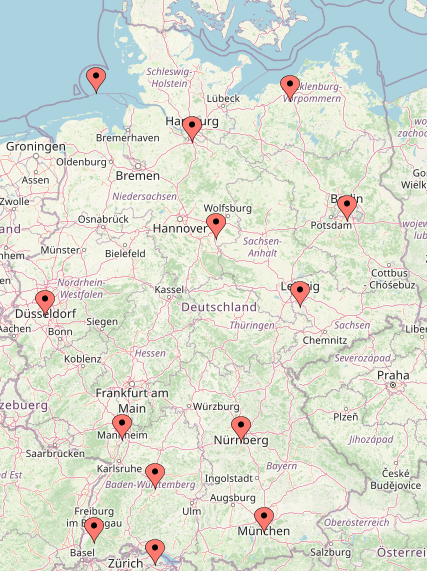
\includegraphics[width=.5\textwidth]{data/stations_map_customizer.png}
            \caption[Weather stations used]{Weather stations used}
            \label{fig::weather_stations}
 \end{figure}
 
\iffalse
\begin{table}[]
\centering
\begin{tabular}{l|l|l}
Station name & Measurements? & MOSMIX ?\\\hline
   Freiburg&Yes&Yes\\
   Hamburg&Yes&Yes\\
    Leipzig-Halle&Yes&Yes\\
    Nuernberg&Yes&Yes\\
    Stuttgart&Yes&Yes\\
    Mannheim&Yes&Yes\\
    Berlin-Tempelhof&Yes&Yes\\
    Duesseldorf&Yes&Yes\\
    Muenchen&Yes&Yes\\
   Konstanz&Yes&Yes\\
   Braunschweig&Yes&Yes\\
   Goettingen&Yes&Yes\\
   Rostock&Yes&Yes\\
   Helgoland&Yes&Yes   
\end{tabular}
\caption{Weather stations used for DWD data}
\label{Table::Weather_Stations}
\end{table}
\fi


 
 
% First explain concepts you used in your thesis like filters or methods
% Then explain your approach or algorithm
% Use flowcharts to give an overview

%\subsection{Additional Data}
%\label{Section::Additional_Data}
%On top of these 3 major thematic fields additional information about working days was used. 

%This data source is expected to capture variations in electricity load.
%School holidays and extended weekends due to public holidays are typical times for taking vacations.
%These effects will be analyzed later in the thesis.

%\subsubsection{Holidays}

%In germany there are static holidays which are always on the same day each year.
%Examples for these are christmas or the 1st of may. 
%Other holidays in germany are dependant on the date of easter. 
%An example for such a holiday is the feast of ascension, which always happens 39 days after easter.

%The bundesAPI provides an api to get information to get this information \cite{HolidayAPIUrl}.

%\subsubsection{School Holidays}

%Information about school holidays is provided by Schulferien.org \cite{SchoolHolidays}. 
%The data is displayed in a table on this website. 
%A webscraper is used to get the data.

\section{Evaluation metrics}
\label{Section:Evaluation_Metrics}

To evaluate the performance of the forecasting models, four metrics are used: two for deterministic accuracy and two for probabilistic forecast quality. This allows for a comprehensive assessment of both point forecasts and prediction intervals.

\subsection{Mean squared error (MSE) and Root Mean Squared Error (RMSE)}

The Mean Squared Error (MSE) and Root Mean Squared Error (RMSE) are used.
This metric is calculated using the formula $MSE = \frac{1}{n} \sum_{i=1}^{n}(Y_i - \hat{Y}_i)^2$
Due to the quadratic nature of this function large errors are penalized harder.

The RMSE is calculated using the formula $RMSE = \sqrt{MSE}$.
By taking the square root of the MSE the value for RMSE is in the same unit as the prediction values. 
This makes the RMSE easier to compare and interpret.

\subsection{Mean average error (MAE)}
The mean average error (MAE) is calculated using $MAE = \frac{1}{n} \sum_{i=1}^{n}|Y_i - \hat{Y}_i|$.
MAE measures the average magnitude of prediction errors, regardless of direction:
Unlike MSE, all deviations are treated equally.

This metric is in the same unit as the prediction values, making it easy to interpret.

\subsection{Continuous Ranked Probability Score (CRPS)}
CRPS evaluates the quality of probabilistic forecasts by comparing the predicted distribution to the actual outcome. In this thesis, it is approximated via pinball loss across a quantile grid: $CRPS = \frac{1}{R} \sum_{\tau\in r} PB_{\tau}$. 
This is calculated for a grid of probabilites $r$ between 0 and 1 of size $R$.
For the evaulation of the experiments $r=\{0.01, 0.02, ..., 0.99\}$ is used, resulting in $R=99$.

The formula for the pinball loss used to approximate the CRPS is $PB_{\tau} = (\tau - \mathbf{1}_{\{Y - \hat{Q}_{\tau}\}}) (Y-\hat{Q}_{\tau}) $,
where $\hat{Q}_{\tau}$ is a forecast of the $\tau -th$ quantile.

\subsection{$\tau$ \% coverage}
This metric measures the share of true values lying within a central prediction interval of width  $\tau$ .
The $\tau$ \% coverage is calculated by chosing a selecting a fraction for $\tau$ and inserting it into the formula $\tau\%-cov = \frac{1}{N} \sum_{i=1}^{N} \mathbf{1}_{\{\hat{Q}_{(1-\tau)/2} < Y_i < \hat{Q}_{(1+\tau)/2} \}}$
where $Y_i$ is the true value for datapoint $i$ and  $\hat{Q}_{\tau}$ is the $\tau -th$ quantile of all forecasts.

\section{Benchmark}
\label{Section:Benchmark}

In addition to comparing models against each other, this thesis uses the Intraday Index ID1 as a baseline benchmark. The ID1 reflects the volume-weighted average price of trades conducted on the intraday market up to one hour before delivery.

This index is used by market participants as a reference point for their final trading decisions and can be interpreted as a proxy for their implicit forecast of the imbalance price.

As explained in Section \ref{Section::Module_2} , the trades happening close to delivery time also play a formal role in Module 2 of the imbalance price calculation. In about 17\% of all settlement periods (2024), the imbalance price was directly influenced by the ID AEP value via the incentivizing component.

While the ID1 represents a strong and practical heuristic, it does not incorporate physical grid variables, weather uncertainty, or reserve activation data. Therefore, one objective of this thesis is to evaluate whether modern time series models can outperform this heuristic baseline under realistic forecasting conditions.


%During the experiments part of this thesis the models will be compared against each other.
%Another benchmark the models will be measured against is the intraday index ID1.
%The intraday index ID1 can be interpreted as a proxy for the market participants' forecast of the imbalance price.

%In a system that is short of energy, a trade for a price higher than the imbalance price would not make sense for a market participant fiscally.
%If no power is bought and instead balancing energy is used the imbalance price has to be paid. 
%As in this scenario the trade would cost more than receiving balancing energy, profit can be made by receiving balancing energy.

%As mentioned in section \ref{Section::Module_2} sometimes the imbalance price is set using the average price of the most recent prices.
%This incentive component was the price setting module only $17.23\%$ of the time in 2024.
%The most recent intraday price still is a very good and simple model \cite{narajewskiProbabilisticForecastingGerman2022}.


\end{document}
